\documentclass{article}[11pt]

\usepackage[spanish]{babel}
\usepackage[utf8]{inputenc}
\usepackage{hyperref}
\usepackage{graphicx}


\author{Pablo Martínez Calatayud}
\title{Práctica 3 - EM}

\begin{document}

\maketitle
\tableofcontents

\newpage

\section{Burkina Faso}
En primer lugar he decido elegir a Burkina Faso ya que creo que es un país muy desconocido para la mayoría de personas. 

\begin{figure}[h]
    \centering
        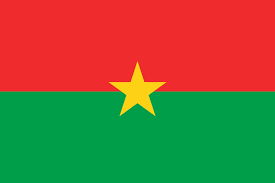
\includegraphics[scale=0.2]{images.png}
        \caption{Bandera de Burkina Faso}
\end{figure}

\subsection{Educación}
Con respecto a la educación en Burkina Faso, el país tiene una tasa del $78,13 \%$ de estudiantes de educación básica. Además, el porcentaje de alumnos que continúan con los estudios es del $41,37 \%$ lo que les sitúa en una posición por debajo del resto de países.


\begin{figure}[h]
    \centering
        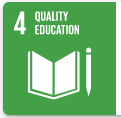
\includegraphics[scale=0.9]{educacion-ods}
\end{figure}

\subsection{Saneamiento y cuidado de las aguas}
    En cuanto al saneamiento e instalaciones burkinesas tenemos que menos de l $47,89 \%$ de la población tiene acceso a agua de una fuente fiable y controlada.
    Burkina Faso se ve muy perjudicada cuando hablamos del tratamiento de aguas residuales ya que no se trata este agua y no parece que se vaya a hacer.

\begin{figure}[h]
    \centering
        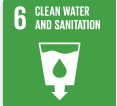
\includegraphics[scale=0.9]{sanitation-ods}
\end{figure}

\newpage

\section{Finlandia}
Finlandia es el país más puntero en términos de los ODS del mundo. La nación finlandesa se encuentra dentro de los conocidos como "países nórdicos", muy reconocidos por su educación y su manera de hacer política. Sus puntos más fuertes son la educación y su sistema de saneamiento. 


\begin{figure}[h]
    \centering
        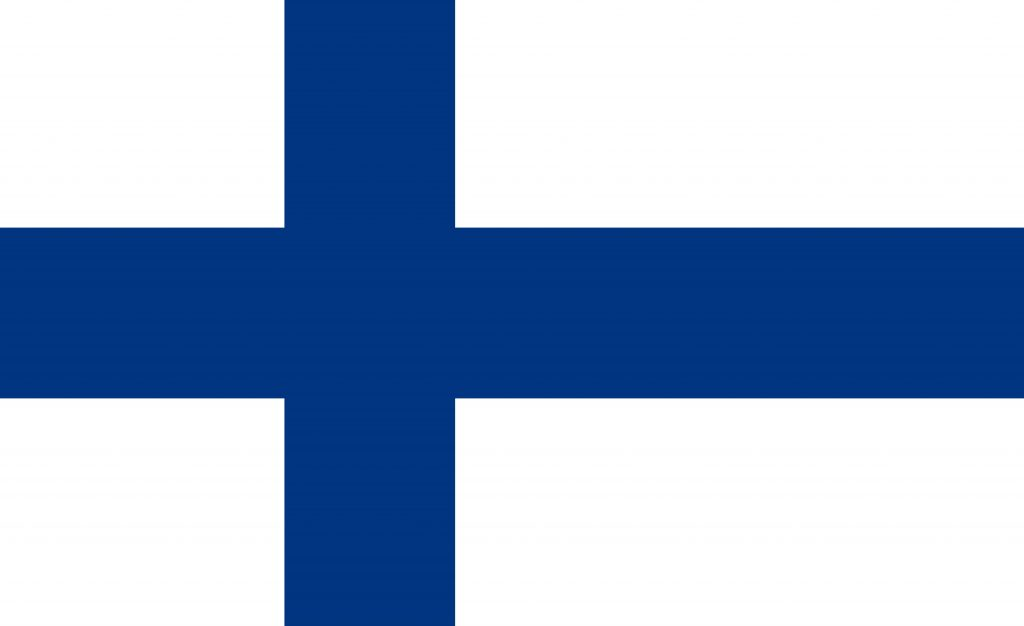
\includegraphics[scale=0.05]{bandera-finlandia.jpg}
        \caption{Bandera de Finlandia}
\end{figure}

\subsection{Educación finlandesa}
En primer lugar, me gustaría hablar de la educación y es que como apuntan los indicadores Finlandia es uno de los países donde más porcentaje de gente decide comenzar a estudiar y se mantiene hasta completar por lo menos la educación secundaria. En concreto, el $98,48 \%$ de la población. Además de esto, también destacan en el índice de educación terciaria, donde el $42 \%$ aproximadamente de la población lo completa. 


\begin{figure}[h]
    \centering
        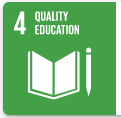
\includegraphics[scale=0.9]{educacion-ods}
\end{figure}

\subsection{Saneamiento y cuidado de las aguas}


En segundo lugar, abordaré el tema del saneamiento y el cuidado de las aguas. El $99,21 \%$ de los habitantes fineses usan instalaciones de saneamiento que se encuentran gestionadas de manera segura, y el total del agua que se utiliza o se trata se recupera y se depura para posterior uso.


\begin{figure}[h]
    \centering
        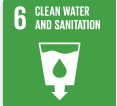
\includegraphics[scale=0.9]{sanitation-ods}
\end{figure}

\newpage

\section{Conclusión}
Para concluir, me gustaría resaltar el gran contraste que hay entre dos países ya que mientras que Finlandia se sitúa en primera posición del ránking de países, Burkina Faso ocupa la posición número 139 de los 165 países que componen el ránking. 

Como podemos ver, Finlandia supera de forma amplia a Burkina Faso en todos los ODS que hemos utilizado para compararlos. El país africano tiene mucho que mejorar y debería tener como ejemplo de como se deben hacer las cosas a Finlandia.
\end{document}
